% !TeX root = ../thuthesis-example.tex

\chapter{Introduction}

\section{Problem definition}

The Internet of Things (IoT) is expected to connect hundreds of billions of devices in less than a decade~\cite{simiscuka_synchronisation_2018}, with tens of billions of connected IoT devices already in existence around the world. This number is anticipated to keep increasing as Internet connectivity has become a standard feature for a significant number of electronic devices~\cite{hu_virtual_2021}. Many companies, such as Huawei, Baidu, Alibaba, Tencent, Google, Intel, etc., already have ways to integrate data coming from IoT devices~\cite{perera}. Although most of these products are restricted for use only with limited types or models of IoT devices, companies may come to standardize IoT devices in the next few years. Nowadays, most consumer IoT devices can be controlled by popular Smart assistants, such as Apple Siri, Amazon Alexa, Tencent Xiaowei, etc., or by SDKs, such as Apple HomeKit~\cite{perera}. Unified solutions make it possible to control all the devices using a phone, computer, or Smart Speaker.
On the other hand, controlling IoT devices by smartphones and Smart speakers does not provide the best user experience. The interaction techniques are limited: even though processing power per energy consumption has increased dramatically, and it is possible to have the processing power of high-performance PC of the 1990s in tiny devices such as smartwatches, there is no freedom of movement and data sharing. Even though 5G networks partly resolve this issue, for example by making it possible to create an Internet of Vehicle (IoV), the transmission bandwidth is still limited, causing severe safety consequences~\cite{hu_virtual_2021}. For example, when computations for interaction techniques such as hand gesture recognition cannot be performed on the IoT device due to its limited computing power, the sensing data must be transferred to a server, analyzed, and only then sent back to the sensing device to provide an output to the user.

The sixth-generation (6G) mobile network is expected to make possible new applications utilizing the increased speed and transmission of the network~\cite{huang_survey_2019, liao_information-centric_2021}. It is expected that a 6G network will be an improvement on the current 5G network and, therefore, provide faster data sharing between devices, which will in turn help overcome the issues stated in the previous paragraph. As soon as this becomes possible, the companies which adapt more quickly to the new standards will be more advanced on the IoT market. Development speed, in this case, is one of the most important factors for companies' success.

Nowadays, the standard ways of integrating newly-developed IoT devices inside the existing environment is to use virtual (or digital) twins or to build prototypes. In the first case, interaction with such devices takes place on a 2D interface, with a very rough simulation of user behavior, which leads to further underestimations of data analysis. In the second case, creating a prototype requires waiting for the IoT device's modeling, sending the schemes to the manufacturers, and then waiting for the prototype to be delivered. In both cases, the disadvantages lead to the possibility of losing market share, either because of lack of usability or because of being too late to enter a market already controlled by competitors. Companies and researchers need an instrument to avoid these disadvantages and integrate prototypes of devices inside the existing real-world IoT environment.

In this research, a solution for this issue is proposed: a platform for developing new IoT devices. The following section describes how using another prospective technology can help create the platform defined above.

\section{Research method}

The problem of defining an instrument for researching new types of IoT devices and integrating them in the existing real-world environments, which was introduced in the previous section, requires a solution. The solution must facilitate integration of real-world devices, and, second, interaction with virtual devices.

Like IoT, Virtual reality (VR), together with AR, is considered one of the essential application-level requirements of 6G. Both technologies can effectively utilize the increased speed and transmission of the sixth-generation network. The biggest companies, such as Facebook, invest billions in AR and VR research. Nearly 10000 employees, almost 20\% of the company staff, work on research in this field~\cite{sam_byford_almost_2021}. Research papers applying Virtual reality to almost every area, such as games, education, healthcare, or industry, can already be found.

Companies selling Virtual Reality Headsets provide powerful APIs for integrating their devices inside different 3D engines \footnote{The Virtual reality market and 3D engine to be used in this research are discussed in the next chapter.}. Researchers can use these interfaces to create a platform for interacting with virtual IoT devices.

The idea of this research project is to integrate Virtual reality headsets into the IoT environment. In the 6G era, it will be possible to send large amounts of data with much smaller latency and much higher speed than that of 5G networks. Wi-Fi 6 (802.11ax standard) already provides acceptable high-quality streaming from VR headsets to the server, with minimal latency in local scenarios.

Nevertheless, only using Virtual reality headsets does not solve the issue defined in the previous section. The research task is to define a layer between a real-world IoT environment and the user as a researcher working to construct new IoT devices (Figure~\ref{fig:VR-IoTResearchPlatformLayer-figure}). The VR-IoT Research Platform is based on this layer. It enables users to perform research on IoT devices inside the IoT-VR environment.

\begin{figure}
  \centering
  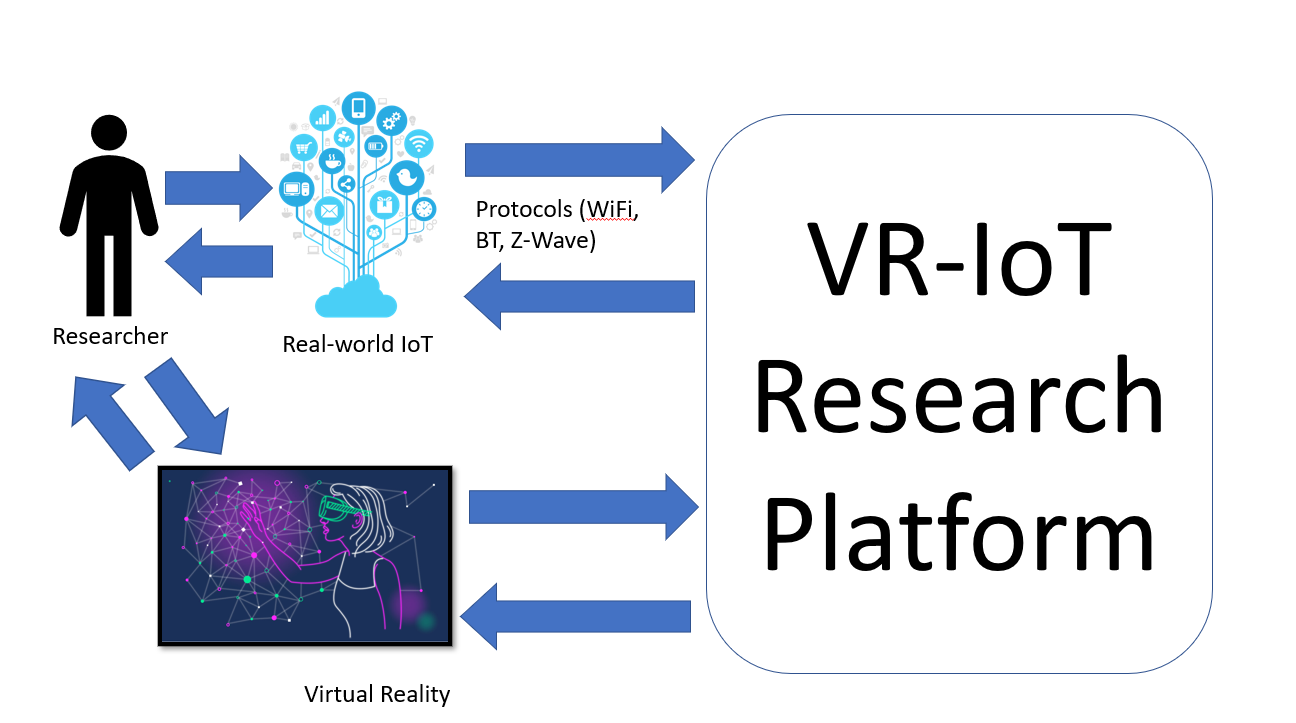
\includegraphics[width=0.9\linewidth]{figures/VR-IoTResearchPlatformLayer.png}
  \caption{VR-IoT Research Platform layer}
  \label{fig:VR-IoTResearchPlatformLayer-figure}
\end{figure}

In Chapter 3, the author proposes a prototype for the platform. In Chapter 4, the prototype is evaluated. In Chapter 5, important assumptions are made about how the platform should be designed in terms of architecture and API to connect to real-virtual world IoT devices. The development cycle and previous prototypes are discussed in Chapter 6. The platform usage examples of existing projects are given in Chapter 7. Chapter 8 includes future directions for inquiry as well as the conclusion.

Summarizing the problem definition and research idea:

\begin{itemize}
    \item Problem definition: There is no instrument for quickly creating, testing, and integrating new IoT devices inside an existing real-world environment.  
    \item Research idea: Define a layer between real-world IoT devices and Virtual Reality. Create a prototype, evaluate its performance and usability, and summarize the outputs. Explain why the selected architecture can be used as the basis for a future product used to design new IoT devices.
\end{itemize}











